\documentclass[tikz,border=10pt]{standalone}
\usepackage{pgfplots}
\pgfplotsset{compat=1.12}

\begin{document}
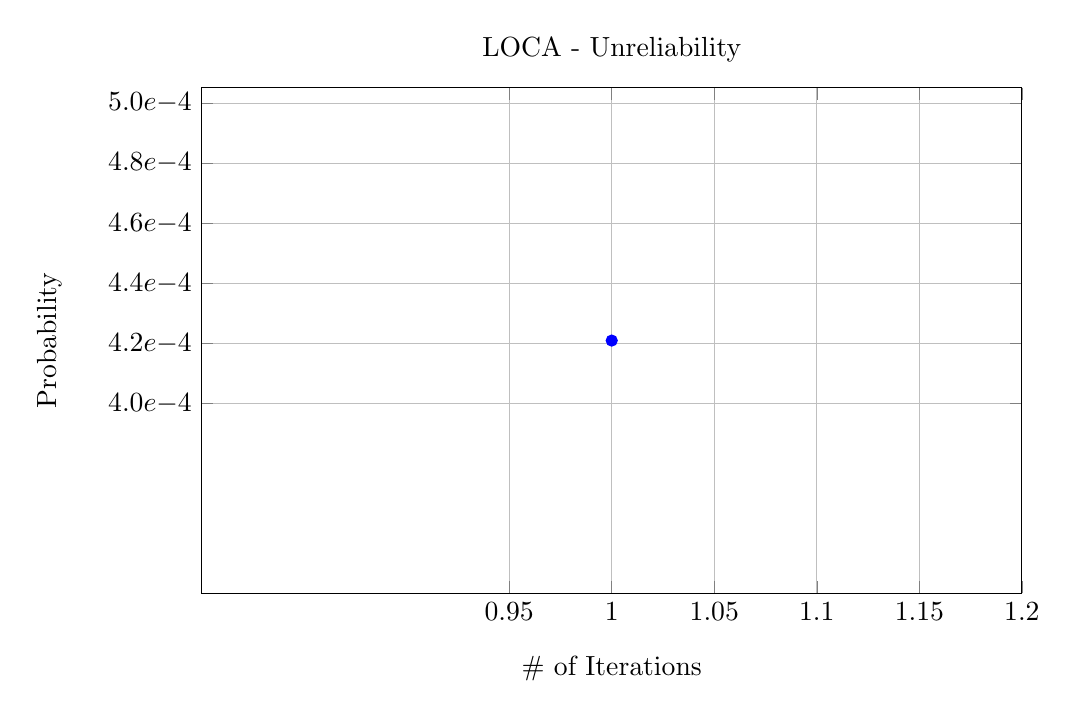
\begin{tikzpicture}
\begin{axis}[
    width=12cm,
    height=8cm,
    title={LOCA - Unreliability},
    xlabel={\# of Iterations},
    ylabel={Probability},
    xlabel style={yshift=-6pt},
    ylabel near ticks,
    ylabel shift=10pt,
    grid=major,
    scaled y ticks=false,
    yticklabel={\pgfmathprintnumber[precision=1,sci,sci e,sci zerofill]{\tick}},
    legend pos=north west,
]
\addplot[color=blue, mark=*] coordinates {
    (1, 0.00042091139193510145)
};
\end{axis}
\end{tikzpicture}
\end{document}
